\documentclass [a4 paper, 11pt, titlepage] {article}

\usepackage{nicematrix}
\usepackage{graphicx}
\usepackage{IEEEtrantools}

\begin{document}
	\title{EE568 Project 4}
	\author{Baris Kuseyri}
	\date{\today}
	\maketitle
	
	\pagenumbering{arabic}
	\tableofcontents
	\newpage
	
	\section{Introduction}

	DW stator topologies are the major stator type used in PMSMs. This is due to their near sinusoidal MMF which yields a high main harmonic winding factor and low torque ripple. It was not until very recently that it was shown that the right choice of slot and pole combination for a FSCW stator could yield a high main harmonic winding factor which is essential to having a high average torque \cite{farshadnia_advanced_2018}









	\subsection{Aims \& Objectives}
	This paper designs an electric motor (EM) to be used as a part of an hybrid electric propulsion system for Cessna 172 Skyhawk. Definition of the hybrid electric propulsion system and the corresponding EM requirements, e.g. rated power, dimensional limitations etc., are outlined in the project proposal. Several EMs with different slot/pole combinations are designed, complying the described requirements. A comparative analysis is performed on these designs, focusing on torque density and cogging torque aspects. One design is chosen, and further alterations are applied to enhance the EM performance. Additionally, this paper proposes a novel winding topology to reduce the cogging torque.


	\section{Literature Review}
	The term FSCW is used to indicate that EM has a non-integral number of slots-per-pole-per-phase $q$,
	\begin{IEEEeqnarray*}{rCl}
		q = \frac{Q}{2pm}
	\end{IEEEeqnarray*}
	where, $Q$ is number of slots, $2p$ is number of poles and $m$ is number of phase.
	
	FSCW topologies are reported to exhibit higher power density. CW comprises of shorter end-windings, resulting with a lower copper loss due to end-windings, compared to DW. FSCW topologies display higher self-inductance, leading to a wider field-weakening region \cite{farshadnia_advanced_2018}.
	The aspect of fault-tolerant in an EM is proportional to several characteristics.
	
	First of all, magnetic coupling between phases, which implies a high mutual inductance, diminishes the fault-tolerancy of an EM. Therefore, phases which are magnetically seperated is desired to achieve a higher fault-tolerancy rating \cite{bianchi_use_2006}. In SPM machines, single-layer winding demonstrates higher self-inductances and lower mutual inductances compared to its double-layer counterparts. A high self-inductance limits the amplitude of short-circuit current, a significant property for fault-tolerancy \cite{el-refaie_fractional-slot_2010} \cite{ishak_comparison_2006}. 
	
	
	Secondly, it is desired to have phases which are physically seperated to achieve fault-tolerancy\cite{bianchi_use_2006}. Lastly, 
	
	
	Mutual coupling between phasesTo achieve a greater fault-tolerant EM
	
	
	Fractional-Slot Concentrated-Winding (FSCW) topology has become of great interest, since it provides a vast amount of choices for the electric motor (EM). 
	
	analytical modelling of the stator MMF and machine equivalent airgap function are essential to correct calculation of the stator magnetic field and inductances, and subsequently torque and torque ripple. analytical formulae for the stator MMF. \cite{farshadnia_advanced_2018}.
	
	\subsection{Torque Density}
	
	\subsection{Torque Ripple}
	3 torque components are present in FSCW PMSM. These are: alignment torque, reluctance torque and cogging torque.
	\begin{IEEEeqnarray*}{rCl}
		T_{em}(t)=T_{align}(t)+T_{rel}(t)+T_{cog}(t)
	\end{IEEEeqnarray*}
	
	Torque generated as a result of the interaction between stator and rotor MMF is alignment torque. $p/2$th harmonic of PM flux linkage, corresponding to fundamental component, contributes to the average alignment torque. Remaining harmonic components provides for the alignment torque ripple \cite{farshadnia_advanced_2018}.
	Torque generated as a result of the stator field aligning the rotor as the reluctance of the magnetic circuit is minimum. Reluctance varies according to the rotor position, while an IPM machine is magnetically salient. This saliency forms as the PM permeability is approximately equals to that of air; thus, contributing to the air-gap length. Similar to alignment torque, $p/2$th harmonic of self and mutual inductance, corresponding to fundamental component, contributes to the average alignment torque. Remaining harmonic components provides for the reluctance torque ripple \cite{farshadnia_advanced_2018}.
	
		
	Cogging torque is one of the torque elements contributing to the torque ripple in the PMSM. Several design factors lead to variation on cogging torque. Here, one such aspect is investigated, that is the amount of stator teeth aligned with poles in the rotor at a given instance. For the corresponding magnetic circuit, permeance is highest when a rotor pole and a stator tooth are aligned. This results with a force that tries to keep the pole steady; hence, emerging a torque counter to the rotor rotation. This is called 'cogging torque'. More of such alignments result with more cogging torque. This description leads to the statement that the value of least common multiple (LCM) of the number of slots $Q$ and number of poles $2p$ is an indicator for the intesity of the cogging torque in a PMSM. LCM of $Q$ and $2p$ is inversely proportional to the cogging torque amplitude \cite{farshadnia_advanced_2018} \cite{zhu_influence_2000}.
	
	
	
	
	
	
	
	
	
	
	FSCW stator topologies are characterized by their slots per pole per phase ratio, denoted $S_{pp}$\cite{farshadnia_advanced_2018}. 
	
	
	
	
	
	
	\section{Analytical Calculation \& Sizing}
	As mentioned in the proposal the machine rating are,
	\begin{table}[h]
		\begin{center}
			\begin{tabular}{c|c|c}
				Power [kW] &  Speed [rad/s] &  Torque [N$\cdot$m]\\
				\hline
				$46.9790$ & $282.7433$ & $166.1542$
			\end{tabular}
		\end{center}
		\caption{Lycoming Operator's Manual IO-360-L2A Operating Conditions}
		\label{fig:EMoperations}
	\end{table}
	

	
	\subsection{Magnetic Loading \& Electrical Loading}
	Permitted RMS values for linear current densities $\bar{A}$, current densities $J$ and peak air-gap flux densities for PMSMs with single-layer field winding, and the corresponding tangential stress $\sigma_{Ftan}$ are reported as follows:
	\begin{table}[h]
		\begin{center}
			\begin{tabular}{c|c|c||c}
				$\bar{A}$ $[kA/m]$ & $\hat{B}_g$ $[T]$ & $J$ $[A/mm^2]$ & $\sigma_{Ftan}$ $[Pa]$ \\
				\hline
				35-65 &  0.85-1.05 & 2-4 & 21000-48000\\
				50 &  0.95 &  & 33876\\
			\end{tabular}
		\end{center}
		\caption{PMSMs with Single-Layer Field Winding }
		\label{fig:EMoperations}
	\end{table}
	Here, $\sigma_{Ftan}$ is calculated by
	\begin{equation}
		\sigma_{Ftan}=\frac{\hat{A}\hat{B}_g}{2}=\frac{\bar{A}\hat{B}_g}{\sqrt{2}}
	\end{equation}
	where, ($\hat{\cdot}$) is for peak value and ($\bar{\cdot}$) is for RMS value of the parameter.
	Therefore, suitable magnetic and electric loading are chosen as
	
	\subsection{Specific Machine Constant}
	\begin{IEEEeqnarray*}{rCl}
		C &=& \frac{\pi^2}{\sqrt{2}}k_w\bar{A}\hat{B}_g=\frac{\pi^2}{2}k_w\hat{A}\hat{B}_g \\
		&=& \frac{\pi^2}{\sqrt{2}}k_w\cdot50\cdot0.95 \\
		&=& 331496.1\cdot k_w [W/m^3]
	\end{IEEEeqnarray*}
	where, $k_w$ is the winding factor.
	
	
	\subsection{Rough Dimensions}
	
	
	\paragraph{Rotor Volume $V_r$} in PMSMs can be calculated in a similar manner with asynchronous machines
	\begin{IEEEeqnarray*}{rCl}
		T &=& \sigma_{Ftan}r_r(2\pi r_rl') \\
		&=& \sigma_{Ftan}V_r \\		
	\end{IEEEeqnarray*}
	\begin{IEEEeqnarray*}{rCl}
		V_r &=& \pi\frac{D^2_r}{2}l'=\frac{T}{2\sigma_{Ftan}} \\
		&=& \frac{166.1542}{2\cdot33876} = 0.0025 [m^3]
	\end{IEEEeqnarray*}

	\paragraph{Air-gap Clearance} in PMSMs can be calculated in a similar manner with asynchronous machines
	\begin{IEEEeqnarray*}{rCl}
		\delta &=& \frac{0.18+0.006P^{0.4}}{1000} [m]=\frac{0.18+0.006\cdot46979^{0.4}}{1000} [m] \\
		&=& 6.235195394489506e-04[m] \\
		&\approx& 0.624 [mm]
	\end{IEEEeqnarray*}
	
	\paragraph{Equivalent Machine Length to Air-gap Diameter $\chi=\frac{l'}{D_g}$} in synchronous machines with pole-pair number more than 1, i.e. $p>1$, this ratio is calculated as
	\begin{IEEEeqnarray*}{rCl}
		\chi &=& \frac{l'}{D_g}\approx\frac{\pi}{4p}\sqrt{p} \\
	\end{IEEEeqnarray*}
	where, the $p$ stands for number of pole pairs in the machine. $\chi$ ratio for different number of pole-pairs $p$ can be seen in Fig. \ref{fig:chiRatio}.
	\begin{figure}[h]
		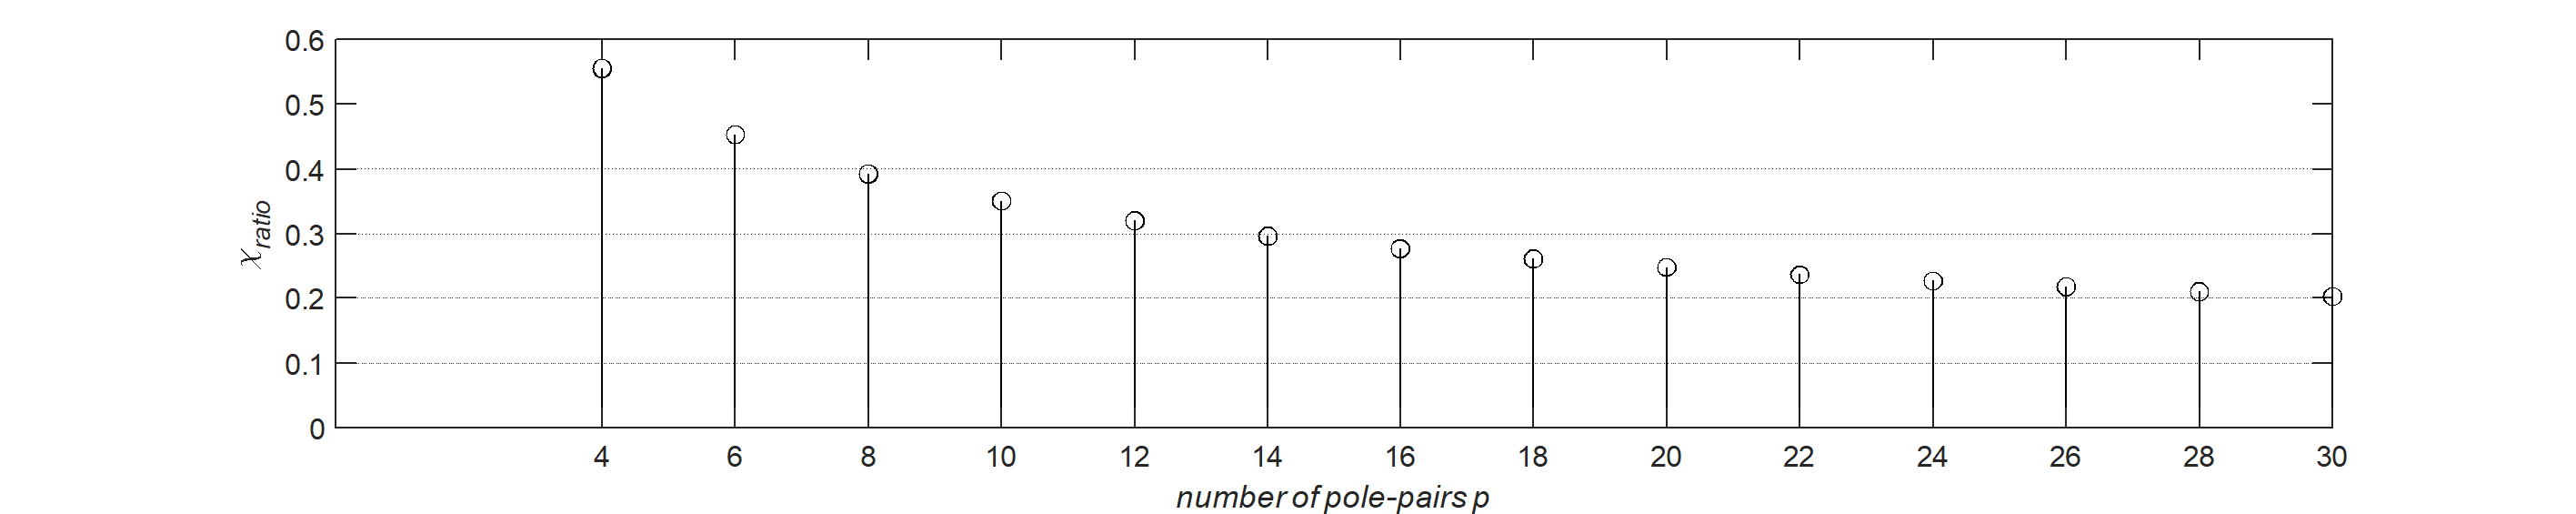
\includegraphics[width=\textwidth]{chiRatio.png}
		\caption{$\chi$ ratio for different number of pole-pairs $p$}
		\label{fig:chiRatio}
	\end{figure}

	
	\begin{table}[h]
		\begin{center}
			\begin{tabular}{c|c}
				 &  \\
				\hline
				airgap clearance & 0.7mm\\
				rotor diameter & 290mm\\
				axial length & 68mm 
			\end{tabular}
		\end{center}
		\caption{Rough Dimensions}
		\label{tab:roughDimensions}
	\end{table}
	
	
	
	
	\subsection{Winding Configurations}
	This paper analyses single-layer FSCW winding configurations. In this manner, topologies with number of slots as $Q=18, 24$, and number of poles as $2p=16, 20, 22, 26, 28$ are inspected. These slot/pole combinations and their corresponding winding factors are presented in Table \ref{tab:windingConf}.
	\begin{table}[h]
		\begin{center}
			$\begin{NiceArray}{|C|C|C|C|C|}[first-row,first-col]
				Q/2p & 16 & 20 & 22 & 26 & 28 \\
				\hline
				18 & 0.945 & 0.945 & 0.902 & 0.735 & 0.617 \\
				\hline
				24 & 0.866 & 0.966 & 0.958 & 0.958 & 0.966 \\
				\hline
			\end{NiceArray}$
		\end{center}
		\caption{Winding Configurations}
		\label{tab:windingConf}
	\end{table}	
	
	\begin{table}[h]
		\begin{center}
			\begin{tabular}{c|c}
				 &  \\
				\hline
				number of slots & \\
				number of coils & \\
				cable size & 
			\end{tabular}
		\end{center}
		\caption{Winding Configurations}
		\label{tab:windingConfigurations}
	\end{table}
	
	
	
	
	
	\subsection{Machine Parameters}
	
	\paragraph{teeth/slot dimensions}
	
	\paragraph{back-core thickness}
		\begin{table}[h]
		\begin{center}
			\begin{tabular}{c|c}
				 &  \\
				\hline
				back-core thickness & 19.07mm \\
				number of coils & \\
				cable size & 
			\end{tabular}
		\end{center}
		\caption{Machine Parameters}
		\label{tab:machineParameters}
	\end{table}
	
	
	
	
	
	
	
	
	
	\subsection{Material selection}
	
	\paragraph{Magnet Material} There are no cost limitations to the EM application. Eclipse Magnetics inform that N35 grade NdFeB magnets have the VH/AH choice, in which the magnet can operate up until the temperatures of $230^{\circ}C$. This is not a requirement for the application, however, implementing N35 PM magnets omits the machine's operable temperature range dependency to the PM magnet demagnetization due to heat.
	N35 grade NdFeB magnet characteristics are given in Table. \ref{tab:N35}
	
	\begin{table}[h]
		\begin{center}
			\begin{tabular}{c|c|c}
				$B_r$ [$mT$] & $H_c$ [$kA/m$] & Max. Energy BHMax [$kJ/m^3$] \\
				\hline
				1170 & 867 & 263
			\end{tabular}
		\end{center}
		\caption{N35 grade NdFeB PM characteristics}
		\label{tab:N35}
	\end{table}
	where, $B_r$ is remanence flux density and $H_c$ is coercivity.
	
	\paragraph{Lamination Material}
	
	
	\begin{table}[h]
		\begin{center}
			\begin{tabular}{c|c}
				 &  \\
				\hline
				back-core thickness & 19.07mm \\
				number of coils & \\
				cable size & 
			\end{tabular}
		\end{center}
		\caption{Material selection}
		\label{tab:materialSelection}
	\end{table}
	
	
	
	
	
	
	
	
	\subsection{Electrical circuit parameter}
	
	

	

	

	

	
	
	
	
	
	
	
	
	\section{FEA Modelling}
	\section{Comparison \& Discussion}
	\section{Conclusion}


	\section{Draft}
	1\cite{alberti_theory_2011}
	2\cite{babitsky_investigation_2019}
	3\cite{boglietti_electrical_2014}
	4\cite{carraro_design_2018}
	5\cite{choi_reduction_2016}
	6\cite{dajaku_advanced_2019}
	7\cite{el-refaie_advanced_2014}
	8\cite{el-refaie_fractional-slot_2010}
	9\cite{el-refaie_fractional-slot_2013}
	10\cite{farshadnia_advanced_2018}
	11\cite{farshadnia_detailed_2016}
	12\cite{geun-ho_lee_torque_2008}
	13\cite{guemes_comparative_2010}
	14\cite{han_torque_2007}
	15\cite{he_evaluation_2019}
	16\cite{howell_getting_2018}
	17\cite{jussila_guidelines_2007}
	18\cite{masmoudi_design_2019}
	19\cite{reddy_generalized_2014}
	20\cite{seok-hee_han_torque_2010}
	21\cite{yokoi_general_2016}
	22\cite{zhu_analysis_2018}
	23\cite{zhu_novel_2019}
	24\cite{zuopeng_design_2017}
	\newpage
	
	\bibliography{bibliography} 
	\bibliographystyle{ieeetr}
\end{document}